
\documentclass[answers]{exam}
%%%%%%%%%%%%%%%%%%%%%%%%%%%%%%%%%%%%%%%%%%%%%%%%%%%%%%%%%%%%%%%%%%%%%%%%%%%%%%%%%%%%%%%%%%%%%%%%%%%%%%%%%%%%%%%%%%%%%%%%%%%%%%%%%%%%%%%%%%%%%%%%%%%%%%%%%%%%%%%%%%%%%%%%%%%%%%%%%%%%%%%%%%%%%%%%%%%%%%%%%%%%%%%%%%%%%%%%%%%%%%%%%%%%%%%%%%%%%%%%%%%%%%%%%%%%
\usepackage{amssymb}
\usepackage{amsmath}
\usepackage{pdfpages}
\usepackage{marvosym}
\usepackage{hyperref}
\usepackage{enumitem}
\usepackage{tikz}
\usepackage{graphicx}
\usepackage{float}
\usepackage{soul}
\usepackage{multirow}

\setcounter{MaxMatrixCols}{10}
%TCIDATA{OutputFilter=LATEX.DLL}
%TCIDATA{Version=5.00.0.2552}
%TCIDATA{<META NAME="SaveForMode" CONTENT="1">}
%TCIDATA{LastRevised=Wednesday, February 16, 2011 02:52:30}
%TCIDATA{<META NAME="GraphicsSave" CONTENT="32">}
%TCIDATA{Language=American English}

\topmargin=-1.8cm \textheight=23.8cm \oddsidemargin=-0.3cm
\evensidemargin=-0.5cm \textwidth=17.1cm
\newtheorem{ass}{Assumption}
\newtheorem{prop}{Proposition}
\newtheorem{thm}{Theorem}
\newtheorem{lem}{Lemma}
\newtheorem{conj}{Conjecture}

\begin{document}


\thispagestyle{empty}\baselineskip1.2\baselineskip\

\noindent \textbf{Econ 140\newline
Summer 2022 \newline
Instructor: Fernando Hoces de la Guardia \newline
GSIs: Elena Stacy \& Yige Wang
}

\vskip2ex

\noindent \textbf{Midterm Exam 1}

\vskip3ex

\noindent \textbf{Thursday July 7, 2022}

\vskip9ex

\vskip9ex


\noindent \textbf{Exam Instructions:}


\begin{itemize}
\item \textbf{You have 80 minutes to answer this exam} 

\item \textbf{This exams has a total of 80 points (suggesting the length of time to spent in each question). Each question indicates the number of points, and indicates a maximum length for its answer} 

\item \textbf{Most questions ask for short answers (from a couple of words, to one or two sentence maximum)} 
\item \textbf{Explanation in black or blue ink is recommended as these often scan the best.} 
\item \textbf{You must submit your solutions using the exam packet provided.} 
\item \textbf{Do not write your solutions on pages that say ``Do not write solutions on this page"}. Answers written on these pages will not be graded. You may use these pages as scratch paper.
\item \textbf{When time is called, STOP} writing, immediately \textbf{CLOSE} your exam packet and hold it up until it is collected.
\item \textbf{Show your work}. Credit will only be awarded on the basis of what is written on the exam.
\item \textbf{Sign the academic honesty pledge}. Cheating will be punished.
\end{itemize}

\newpage

\vspace{2.5in}

\noindent Student Name:

\vskip5ex

\noindent Student ID Number:

\vskip10ex

\noindent \textbf{Affirm the academic honesty pledge below}. For those writing on a non-printed copy, please just write ``Academic Honesty Pledge as on exam'', and sign your name. \\\textbf{\underline{If you do not affirm this pledge, your exam will be marked invalid.}}


\vskip12ex

\noindent \textbf{0. ACADEMIC HONESTY PLEDGE }

\noindent I confirm that I have abided by all academic honesty rules for UC Berkeley and Economics 140. I confirm that I did not see this exam before my official exam start time. I confirm that I have not shared and will not share this exam with anyone else. I confirm that I haven't copied from anybody else's exam.

\vskip5ex

Signature: \hrulefill

\vskip5ex


\newpage

%\noindent \textbf{1. Short Questions (15 points, 3 points per question.)}

\vskip1ex

\begin{enumerate}

	\item  Based on our class discussion of the concept of bullshit: what is the key characteristic that distinguishes bullshit from lies (or the bullshitier from the liar) [2pt, 1-2 sentences].   
	
	\begin{solution}
	Bullshiters are indifferent or ignorant between true facts and lies, while liars are aware of and intentionally make false claims.
	\end{solution}
	







	\item How can we compute the probability of an event for the case of a continuous random variable? [2pt, 1 sentence] 
	\begin{solution}
	Compute the area under the probability density function curve where the event lies.
	\end{solution}
	

	\item For the case of a continuous random variable: which distribution is a good representation of not knowing much about a phenomenon (represented by the random variable)? How about for a discrete random variable (assume 2 events for simplicity)?
	[2pt, 2 sentences]
	\begin{solution}
	UPDATEDThe uniform distribution is a good starting point when we are ignorant, since it simply assumes that each event (of equal range) is equally likely to occur.  In the discrete case with two events, ignorance could be reflected by a probability of 50\% for each outcome (Bernulli distribution).
	\end{solution}


\item 
    The probability that two random variables, $X, Y$ take the values of $x$, \textbf{and} $y$ can \textbf{always} be described as: [2pt]
    \begin{enumerate}[label=\alph*)]
    \item  $\operatorname{Pr}(\mathrm{X}=\mathrm{x})+(\mathrm{Y}=\mathrm{y})$
    \item $\operatorname{Pr}(\mathrm{X}=\mathrm{x}, \mathrm{Y}=\mathrm{y})$.
    \item $\operatorname{Pr}(\mathrm{X}=\mathrm{x}) *(\mathrm{Y}=\mathrm{y})$
    \item $\operatorname{Pr}(\mathrm{X}=\mathrm{x}) /(\mathrm{Y}=\mathrm{y})$
    \end{enumerate}

 \begin{solution}
 b)
 \end{solution}
 
\item Using the concept of conditional probabilities, the same term as in the question above (the probability that two random variables, $\mathrm{X}, \mathrm{Y}$ take the values of $\mathrm{x}$, and $\mathrm{y})$ can be described as. [2pt]
\begin{enumerate}[label=\alph*)]
    \item $\operatorname{Pr}(\mathrm{X}=\mathrm{x} \mid \mathrm{Y}=\mathrm{y})^{*} \operatorname{Pr}(\mathrm{X}=\mathrm{x})$
    \item $\operatorname{Pr}(\mathrm{Y}=\mathrm{y} \mid \mathrm{X}=\mathrm{x})^{*} \operatorname{Pr}(\mathrm{Y}=\mathrm{y})$
    \item $\operatorname{Pr}(\mathrm{X}=\mathrm{x} \mid \mathrm{Y}=\mathrm{y})^{*} \operatorname{Pr}(\mathrm{Y}=\mathrm{y})$
    \item $\operatorname{Pr}(\mathrm{Y}=\mathrm{y} \mid \mathrm{X}=\mathrm{X})$
\end{enumerate}

\begin{solution}
c)
\end{solution}



\item Define the concept of independence in plain English [4pt, 1-2 sentences]
\begin{solution}
UPDATED Two events are independent if the occurrence of one event does not effect the likelihood of occurrence of the other event. \textit{Alternatively} Two random variable are independent if the learning about the value of one, tell us nothing about the probability of the other. 
\end{solution}

    \item Define the concept of independence in terms of conditional probabilities. [2pt, 1-2 sentences equation] 
    
    \begin{solution}
    $$ P(X=x|Y=y)=P(X=x)$$
    \end{solution}
    



	\item In which sense is the variance, an average. What is an average of? [2pt, 1 sentence]
	
	\begin{solution}
UPDATED	The variance is the average squared distances to the mean.
	\end{solution}
	

	\item Compute the variance for a variable with values 2,3, and 4. Show your calculations. [4pts, 2-5 lines] 
	\begin{solution}
UPDATED
	\begin{align*}
	    \overline{X} & = \frac{2+3+4}{3} = 3 \\
	    & \\
	    \sigma^2 & = \frac{(2-3)^2 + (3-3)^2 + (4-3)^2}{3} \\ 
	    \sigma^2 & = \frac{1 + 0 + 1}{3} \\ 
	    \sigma^2 & = \frac{2}{3}
	\end{align*}
A computation using the ($n-1$) adjustment it's also ok. 
	\end{solution}

	
\newpage
	\item An econometrics class has 75 students, and the mean student weight is 155 lb. A random sample of four students is selected from the class, and their average weight is calculated. 
	\begin{enumerate}
	    \item Will the average weight of the students in the sample equal 155 lb? [1pt, Yes/No] 
\begin{solution}
No.
\end{solution}

    \item Explain why you answered yes or no to the above question. [1pt, 1 sentence] \begin{solution}
	    The sample average will not necessarily equal 155 lb. It will depend on the sample of students that is selected, and how much variation there is in the class weight.
	    \end{solution}
	    \item Is the sample average, $\overline{Y}$ , a random variable? [1pt, 1 sentence] 
	    \begin{solution}
	    UPDATED Yes, the sample average is a random variable because its the sum of a collection of RVs (divided by the sample size)
	    \end{solution}
	\end{enumerate}


	\item In a rectangular data set: what is represented by rows and what by columns.  [1pt, 1 sentence]

\begin{solution}
    Rows represent individual observations, and columns represent variables. 
\end{solution}
	\item Assume that you have received a data set with millions of observations on the income of all the American households. Which concept(s) discussed in class can you use to communicate some initial insights about these millions of observations? [2pt, 1 sentence]

\begin{solution}
    UPDATED Compute the mean and standard deviation of income. Reference to the distribution are OK but not required. 
\end{solution}
	\item What is the interpretation of the mean of a binary variable? [2pt, 1 sentence]
\begin{solution}
    The mean of a binary variable is the proportion of 1's.
\end{solution}

\newpage
	\item What is the main reason we prefer to report (and read) standard deviations instead of variances? [2pt, 1 sentence]
\begin{solution}
    The standard deviation is in the same units as the original values, which makes it much easier to work with and easier to interpret.
\end{solution}

	\item Given a collection of random variables, Y1, Y2, …, Yn let $\overline{Y}$ represent its sample mean. What happens with its expected value as the number of random (n) variables increases. What happens to its variance? [2pt, 1-2 sentences]
\begin{solution}
    UPDATED The expected value does not change, it remains constant. The variance shrinks towards zero. 
\end{solution}

\item Given a data set with information on the age of each individual in the US (360 million), choose which of the following could be a \textbf{plausible} value for the standard deviation\textbf{ of the sample mean}. [2pt]
\begin{enumerate}
    \item -32
    \item 32
    \item 320
    \item 0.32
\end{enumerate}
\begin{solution}
d)
\end{solution}

\item Explain your answer to the above question. [2pt, 1 sentence]
\begin{solution}
  UPDATED The standard deviation of the sample mean shrinks as $n$ increases, hence the only plausible value is 0.32. 
\end{solution}

\item For the simulation performed in class and sections to explore the Central Limit Theorem: 
\begin{enumerate}
    \item What happens with the distribution of the sample mean as we increase the sample size? [4pt, 1-2 sentences]
   \begin{solution}
	UPDATED The distribution becomes normal with an ever shrinking standard deviation. 
	\end{solution}
    \item What happens with the distribution as we increase the number of simulations/draws? [2pt, 1 sentence]
    \begin{solution}
	UPDATED The histogram (or empirical distribution) approximates better the theoretical distribution. 
	\end{solution}
\end{enumerate}


\item Name what is the key assumption that is violated when we observe a spurious correlation. [3pt, 1 sentence]

    \begin{solution}
	Other things equal, aka All else equal, aka ceteris paribus.
	\end{solution}
	
\item Let’s look again at the table used to explain the intuition behind conditional probabilities. Add two new variables “$Pass|S=1$” and “$Pass \text{ \& } S$” and fill-in the corresponding value of each observation [2 columns, 6pts]. 
\begin{figure}[H]
    \centering
    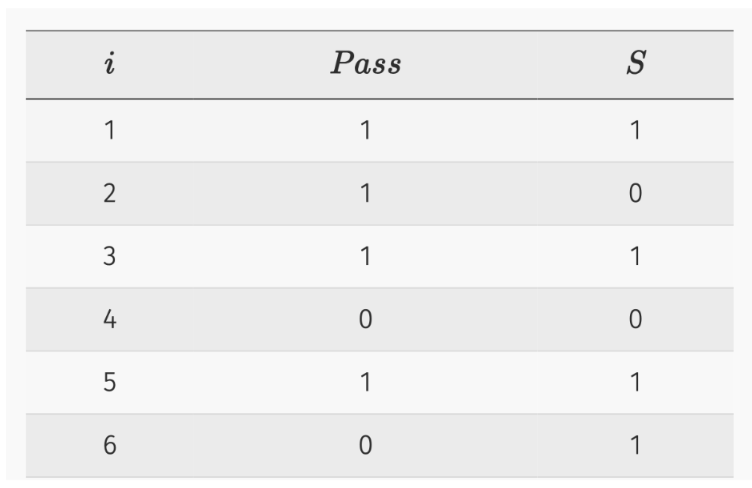
\includegraphics[width=4in]{Figures/midterm_pass.png}
    \caption{}
    \label{}
\end{figure}
\begin{solution}
	\begin{figure}[H]
    \centering
    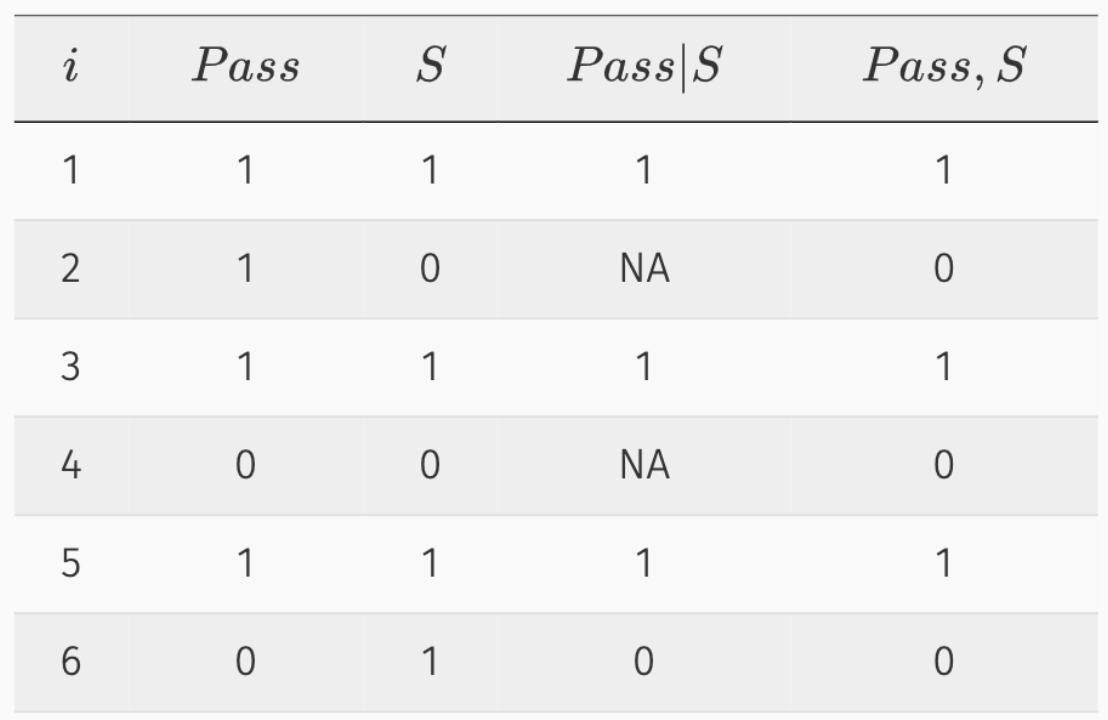
\includegraphics[width=4in]{Figures/midterm_pass_sol.png}
    \caption{}
    \label{}
\end{figure}
	\end{solution}


\item (Modified ``Conditionities''). Annie lives in a town of 3000 individuals where a disease called ``Conditionities'' is scaring the population. The disease affects 2\% of the population and there is a test that detects the disease with 90\% success (meaning that, when a person has the disease, the tests comes positive 90\% of the time; and when the person does not have the disease, it comes negative 90\% of the time). Annie just took a test and it came up positive, what is the probability that the has the disease? [6pt, 2-6 lines] 

[Suggestion: getting stuck in this question might consume a significant portion of your time, if the answer doesn't come to you immediately, leave it for the end]

[Help, in addition to Bayes formula printed on question 27, you might also need the law of total probabilities. This states that for two random variables X and Y, the probability of X taking a specific value can be broken down into the following conditional probabilities:]

\begin{equation}
    P(X=x) = \sum_{i}P(X=x|Y=y_i)P(Y=y_i)
\end{equation}

\begin{solution}
 UPDATE   We want to calculate the conditional probability that Annie has Conditionitis, given that they tested positive. We can solve this with two approaches, one discuss in class, the other in session (both are fine). 
    
    Define RVs $D$ with value 1 if somebody has the disease and 0 otherwise, and $T$ with value 1 if they tested positive and 0 o/w. 
    
    We know: $P(D=1) = 0.02$, $P(T=1|D=1) = P(T=0|D=0) = 0.9$, we want to know $P(D=1|T=1)$. 
    
    Using Bayes formula:  
    
    \begin{aligned}
        P(D=1|T=1) &= \frac{ P(T=1|D=1)P(D=1)}{P(T=1)}\\
        &= \frac{ 0.9 \times 0.02 }{P(T=1)} \text{   with}\\
    P(T=1) &= P(T=1|D=1)P(D=1) + P(T=1|D=0)P(D=0) \\
       P(D=1|T=1) &= \underbrace{\frac{ 0.9 \times 0.02 }{ 0.9 \times 0.02 +  0.1 \times 0.98}}_{\text{full credit up to here}} =\frac{ 0.018 }{0.018 +0.098} \approx \frac{1}{6} = 16\%
    \end{aligned}
    
    
Answers that go only got to the first equality in the last line above, or made mistakes after, still get full credit.     
    
    
    
    Alternatively, we can put together a table based on the information we have, starting by filling in the bottom row (population of 3,000, with a 2\% rate of disease). 
    \begin{table}[H]
        \centering
        \begin{tabular}{c|c|c|c}
             & Diseased & Not Diseased &  \\
            \hline Positive & 54 & 294 & 348 \\ 
            \hline Negative & 6 & 2646 & 2652 \\ 
             \hline & 60 & 2940 & 3000 \\ 
             \hline
        \end{tabular}
        \caption{Caption}
        \label{tab:my_label}
    \end{table}
    We can see here that given a positive test (positive row), the probability of disease is $54/348 = .155$. \\ 
    
\end{solution}


\item Describe the intuition behind balance in pre-treatment variables. [4pt, 1-3 sentences] 
\begin{solution}
UPDATED We evaluate “balance” of observable characteristics across treatment and control groups, to check if some of the "other things" in the other things equal assumption are (roughly) equal. Evidence of difference, or in-balance, in observable characteristics suggest a violation of this assumption also in unobservables. Hence the presence of selection bias.
	\end{solution}


\item Provide a one-line interpretation for all the numbers highlighted in the 2nd row of the following table (one line per box)? [8pt, 3 sentences] 
\begin{figure}[H]
    \centering
    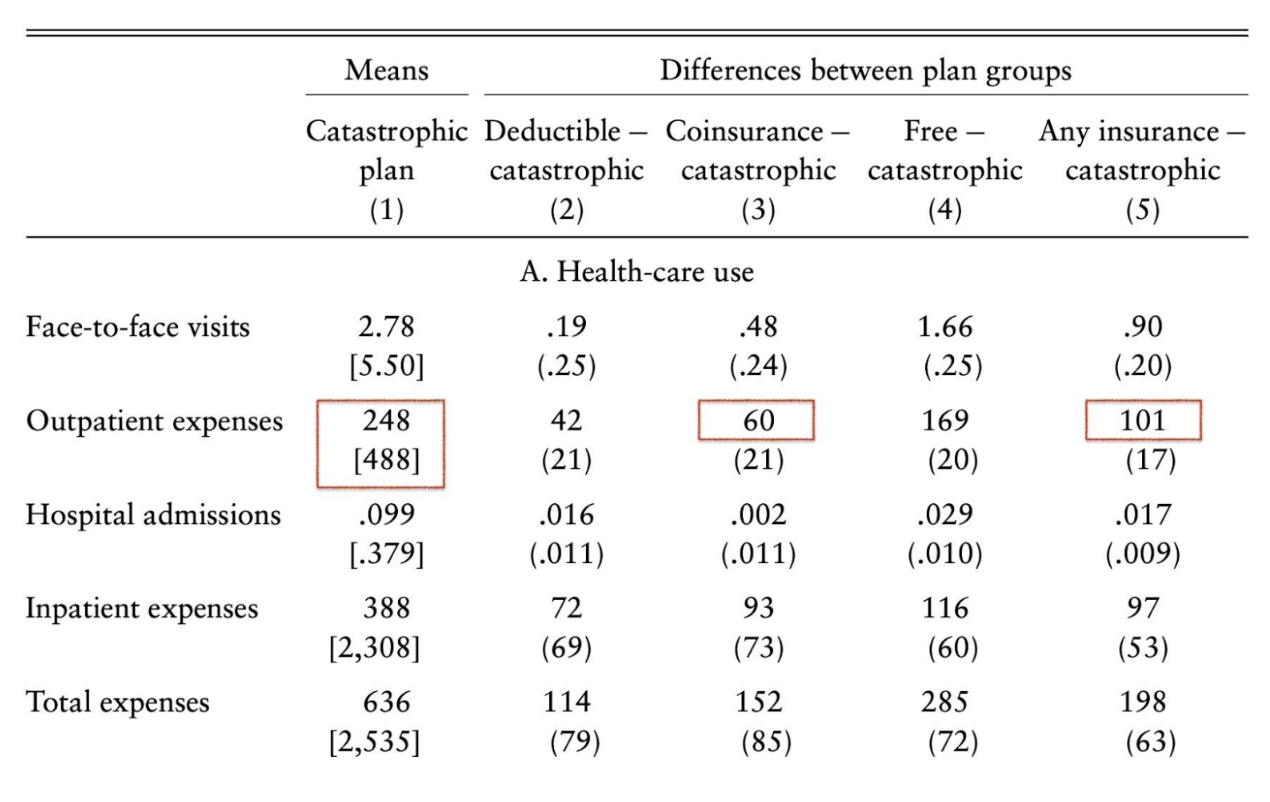
\includegraphics[width=6in]{Figures/midterm_table.png}
    \caption{}
    \label{}
\end{figure}

\begin{solution}
    \\
    Box 1: Outpatient expenses in the Catastrophic plan had a mean of 248 dollars and a standard deviation of 488 dollars. \\ 
    Box 2: Outpatient expenses in the Coinsurance group are 60 dollars higher than those in the catastrophic plan, on average. \\ 
    Box 3: Outpatient expenses in the Any insurance group are 101 dollars higher than those in the catastrophic plan, on average. 
\end{solution}

\item For the exercise of potential outcomes done in class with a fictional data of 10 individuals, cross with an x the potential outcomes that are missing from the data. [6pts, write x's on table] 
\begin{figure}[H]
    \centering
    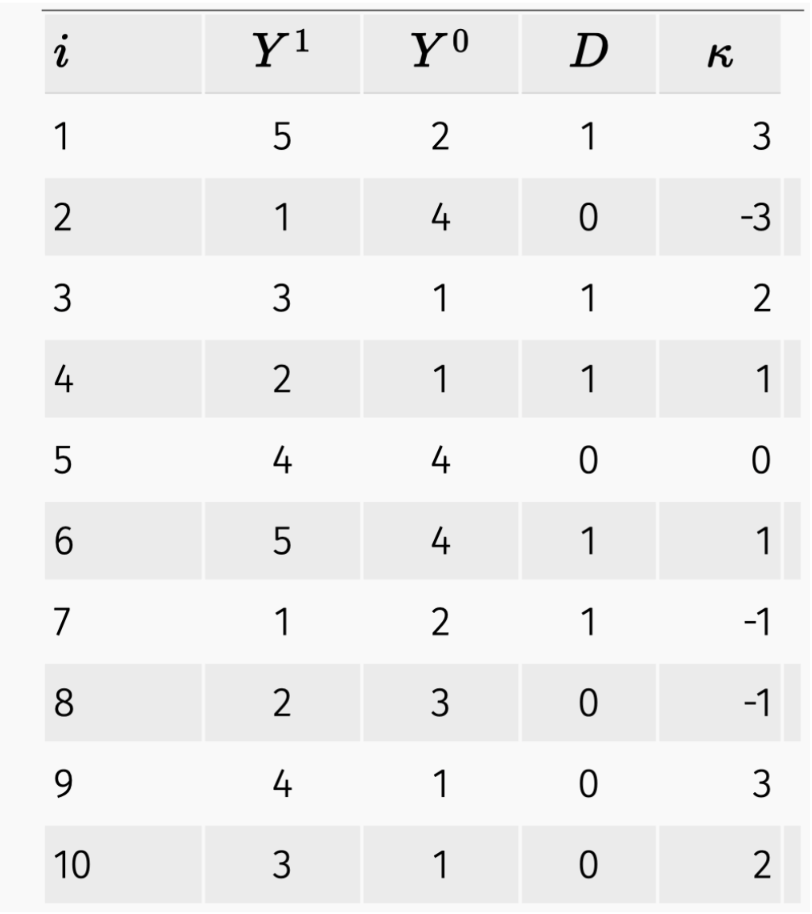
\includegraphics[width=3in]{Figures/midterm_outcome.png}
    \caption{}
    \label{}
\end{figure}
\begin{solution}
NA corresponds to where you should have put an X in the figure below. 
\begin{figure}[H]
    \centering
    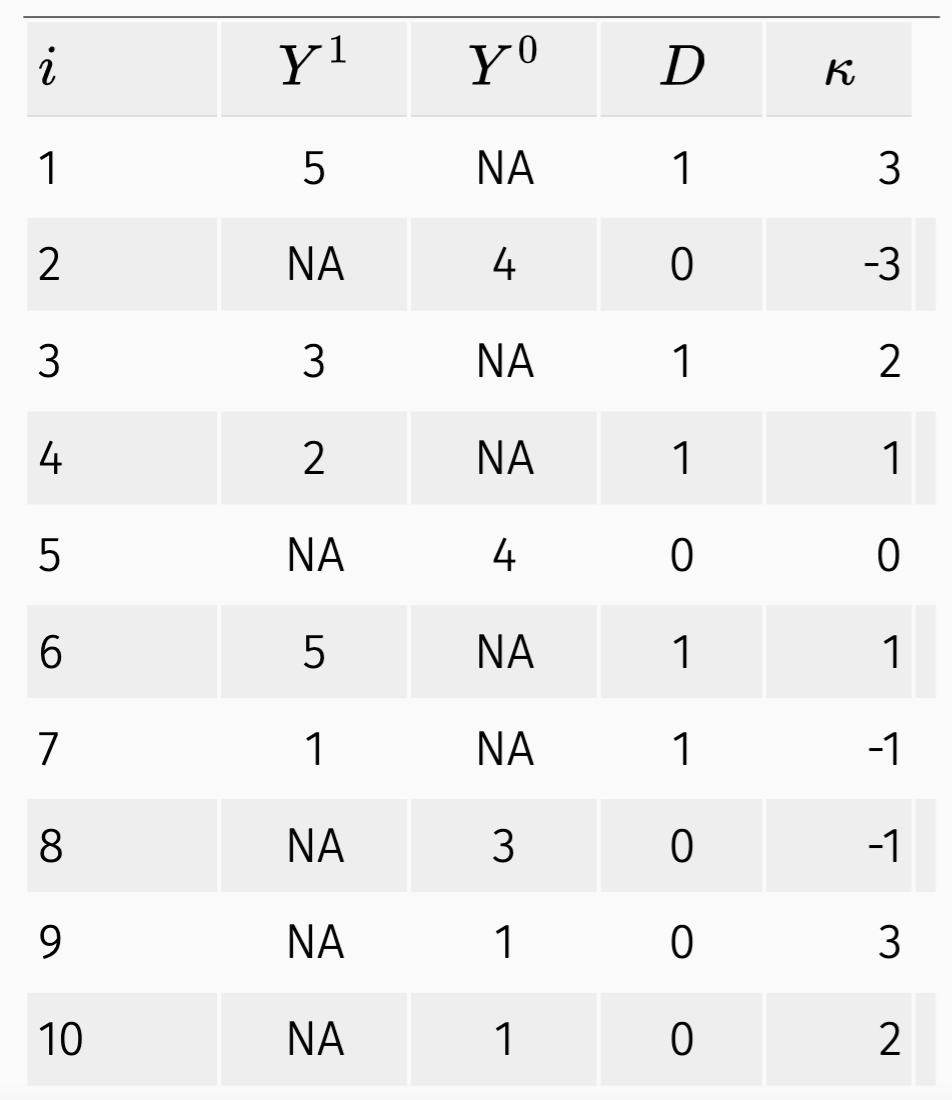
\includegraphics[width=3in]{Figures/midterm_outcome_sol.png}
    \caption{}
    \label{}
\end{figure}
\end{solution}


\item $\mathbb{V}(Y)=\mathbb{E}(\mathbb{V}(Y \mid X))+\mathbb{V}(\mathbb{E}(Y \mid X))$

Ev(v)es Law, the expression above, tells us that the unconditional variance will always be [3pt] : 
\begin{enumerate}
    \item Larger or equal than the conditional variance
    \item Smaller or equal than the conditional variance
    \item Larger when the Y is independent of X
    \item Smaller when Y is independent of X
\end{enumerate}
\begin{solution}
(a)
\end{solution}
\vspace{3cm}
\newpage

\item \textit{[Bonus Question. Suggestion: focus on this question only after you are done with the rest of the exam]}

Monty Hall Problem (slightly modified):
Suppose you're on a game show, and you're given the choice of \textbf{four} doors: Behind one door is a car; behind the others, goats. You pick a door, say No. 1, and the host, \textbf{who knows what's behind the doors}, opens another door, say No. 4, which has a goat. He then says to you, \st{``Do you want to pick door No. 4?''} \textit{``Do you want to change your choice from Door No. 1?''}\footnote{Correction, noted on the board during the exam, update typed here on Jul 7.} Is it to your advantage to switch your choice?\\

Explain the solution to the Monty Hall problem in plain English.[3pts, 1-3 sentences]
\begin{solution}
UPDATED Before Monty opens a door different from yours, each of those doors had a 1/4 chance of having the prize, for a total of 3/4. When he opens a door, given that he knew where the prize was, there still is a probability of 3/4 among the remaining doors (or 3/8 each). This odds are better than your current door, which continues to have a 1/4 (or 2/8) chance of having the prize. 
\end{solution}

\item $[Bonus]$ Derive the solution to the Monty Hall problem using Bayes rule [3pts, 2-6 lines]. 
Reminder of Bayes rule 
\begin{equation}
    P(A|B) = \frac{P(B|A)P(A)}{P(B)}
\end{equation}
\begin{solution}
UPDATED We are interested in the probability the car in door 1, given that Monty open door 4 $(P(\text{Car 1}| \text{Monty 4}))$. Using Bayes: 

\begin{equation}
    P(\text{Car 1}| \text{Monty 4}) = \frac{ P(\text{Monty 4} | \text{Car 1}) P(\text{Car 1})}{P(\text{Monty 4})}
\end{equation}


\begin{itemize}
    \item If the car is in 1, Monty has a 1/3 chance of picking door 4. Hence $P(\text{Monty 4} | \text{Car 1}) = 1/3$. 
    \item The unconditional probability of car being in 1, $P(\text{Car 1})$, is 1/4. 
    \item The probability of Monty choosing is equal probability of any door, after discarding the one that contains the prize, so$P(\text{Monty 4}) = 1/3$
\end{itemize}
Given this:
\begin{equation}
    P(\text{Car 1}| \text{Monty 4}) = \frac{1/3 \times 1/4 }{1/3} = 1/4
\end{equation}

Given that the probability of winning if you stay is 1/4, and 3/8 if you switch (3/4 split equally among the other two doors), you should always switch. 
\end{solution}
\end{document}
